%---------------------------------------------------------------------------
%	PACKAGES AND OTHER DOCUMENT CONFIGURATIONS
%---------------------------------------------------------------------------
\documentclass[final]{beamer}
\usepackage{gensymb}
\usepackage{textcomp}
\usepackage{overpic}
\usepackage[scale=1]{beamerposter} % Use the beamerposter package for laying out the poster
\usetheme{confposter} % Use the confposter theme supplied with this template
\setbeamercolor{block title}{fg=jblue,bg=white} % Colors of the block titles
\setbeamercolor{block body}{fg=black,bg=white} % Colors of the body of blocks
\setbeamercolor{block alerted title}{fg=white,bg=jblue} % Colors of the highlighted block titles
\setbeamercolor{block alerted body}{fg=black,bg=jblue!10} % Colors of the body of highlighted blocks
% Many more colors are available for use in beamerthemeconfposter.sty
%---------------------------------------------------------------------------
% Define the column widths and overall poster size
% To set effective sepwid, onecolwid and twocolwid values, first choose how many columns you want and how much separation you want between columns
% In this template, the separation width chosen is 0.024 of the paper width and a 4-column layout
% onecolwid should therefore be (1-(# of columns+1)*sepwid)/# of columns e.g. (1-(4+1)*0.024)/4 = 0.22
% Set twocolwid to be (2*onecolwid)+sepwid = 0.464
% Set threecolwid to be (3*onecolwid)+2*sepwid = 0.708

% user defined
\usepackage{bm}
\newlength{\sepwid}
\newlength{\onecolwid}
\newlength{\twocolwid}
\newlength{\threecolwid}
\setlength{\paperwidth}{48in} % A0 width: 46.8in
\setlength{\paperheight}{36in} % A0 height: 33.1in
\setlength{\sepwid}{0.024\paperwidth} % Separation width (white space) between columns
\setlength{\onecolwid}{0.1386667\paperwidth} % Width of one column
\setlength{\twocolwid}{0.3013333\paperwidth} % Width of two columns
\setlength{\topmargin}{0.0in} % Reduce the top margin size

\newcommand{\Reals}{\mathbb{R}}
\newcommand{\summ}{\mathbb{S}}
\newcommand{\la}{\leftarrow}
\newcommand{\ra}{\rightarrow}
\newcommand{\lra}{\leftrightarrow}
\newcommand{\bd}{\bm{d}}
\newcommand{\bz}{\bm{z}}
\newcommand{\btheta}{\bm{\theta}}
\newcommand{\target}{\bm{I}_t}
\newcommand{\synth}{\bm{I}_s}
\newcommand{\bsigma}{\bm{\Sigma}}
\newcommand{\fsigma}{\sigma_f}
\newcommand{\fsigmax}{\sigma_{fx}}
\newcommand{\fsigmay}{\sigma_{fy}}
\newcommand{\fscale}{c_f}
\newcommand{\light}{E}
\newcommand{\bx}{\bm{x}}
\newcommand{\by}{\bm{y}}
\newcommand{\bom}{\bm{\omega}}

\newcommand{\toptext}[2]{$\overbrace{\hspace{#1}}^{\text{\normalsize #2}}$}

\DeclareMathOperator*{\argmin}{arg\,min}
\DeclareMathOperator*{\argmax}{arg\,max}

\newlength{\resultwidth}
\setlength{\resultwidth}{1.5in}

%---------------------------------------------------------------------------
\usepackage{graphicx}  % Required for including images
\usepackage{booktabs} % Top and bottom rules for tables
%---------------------------------------------------------------------------
%	TITLE SECTION 
%---------------------------------------------------------------------------
\title{A Bayesian Inference Framework for Procedural Material Parameter Estimation} % Poster title
\author{Yu Guo$^1$, Milo\v{s} Ha\v{s}an$^2$, Lingqi Yan$^3$ and Shuang Zhao$^1$} % Author(s)
\institute{$^1$University of California, Irvine \hspace{2cm}
$^2$Adobe Research \hspace{2cm}
$^3$University of California, Santa Barbara
\vspace{1cm}
% \textbf{}\Large{ACM Transactions on Graphics (SIGGRAPH Asia 2018), 37(6), 2018}
} % Institution(s)
%----------------------------------------------------------------------------
\begin{document}

\begin{frame}[t] % The whole poster is enclosed in one beamer frame
\vspace{-1.5cm}
\begin{columns}[t] % The whole poster consists of three major columns, the second of which is split into two columns twice - the [t] option aligns each column's content to the top
    %----------------------------------------------------------------------------
    %	LEFT
    %---------------------------------------------------------------------------
    \begin{column}{\sepwid}\end{column} % Empty spacer column
    \begin{column}{\twocolwid} % The first column
        \begin{block}{Introduction}
            \large{
                Procedural material models have been graining traction in many applications thanks to their flexibility, compactness, and easy editability.
                In this paper, we explore the inverse rendering problem of procedural material parameter estimation from photographs using a Bayesian framework.
                We use \emph{summary functions} for comparing unregistered images of a material under known lighting, and we explore both hand-designed and neural summary functions. In addition to estimating the parameters by optimization, we introduce a Bayesian inference approach using Hamiltonian Monte Carlo to sample the space of plausible material parameters, providing additional insight into the structure of the solution space.
                To demonstrate the effectiveness of our techniques, we fit procedural models of a range of materials---wall plaster, leather, wood, anisotropic brushed metals and metallic paints---to both synthetic and real target images (See Results section).
                \vspace{1cm}
            }
            
            \begin{figure}
                \includegraphics[width=0.9\linewidth]{images/other/teaser.jpg}
             	\caption{\label{fig:teaser}
             		A scene rendered with material parameters estimated using our method: bumpy dielectrics, leather, plaster, wood, brushed metal, and metallic paint. The insets show a few examples of the initial flash photograph, and our procedural material with parameters found by posterior maximization.}
             \end{figure}
    
        \end{block}
        
        \vspace{2cm}
        
        \begin{block}{Framework}
            \large{
                We implement the procedural generation and rendering processes as (differentiable) PyTorch procedures with the priors and summary functions (classical or neural) expressed in the same framework. These four components (priors, procedural material model, rendering, summary function) together define our posterior distribution, a rather complex (but fully differentiable) function.
            }
            \begin{figure}[t]
            	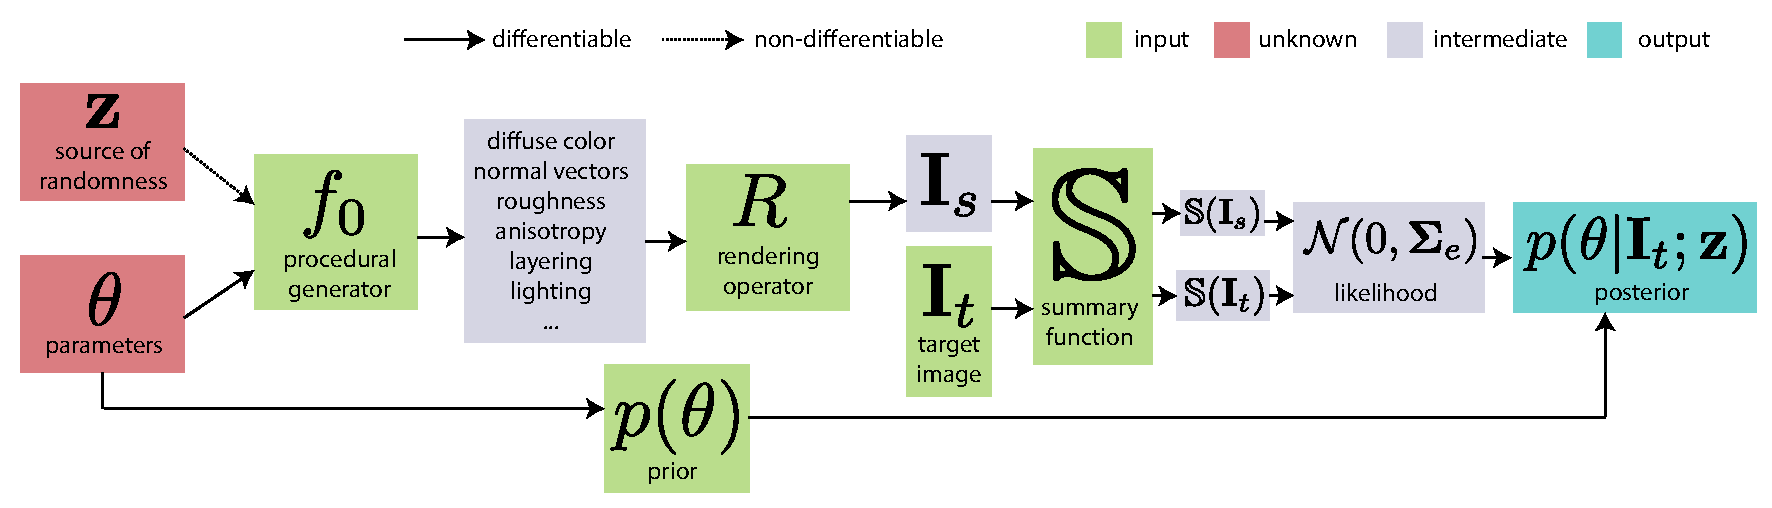
\includegraphics[width=\textwidth]{images/other/framework.pdf}
            \end{figure}
        \end{block}
    \end{column} % End of the first column
    
    %----------------------------------------------------------------------------
    %        MIDDLE
    %----------------------------------------------------------------------------
    \begin{column}{\sepwid}\end{column} % Empty spacer column
    \begin{column}{\twocolwid} % Begin a column which is two columns wide (column 2)
        \begin{block}{Methods}
        \large{
            \textbf{Forward evaluation:}
            \begin{equation*}
                f(\btheta; \bz) := R(f_0(\btheta; \bz))
            \end{equation*}
            Our forward evaluation contains procedural material generation $f_0$, and standard rendering process $R$. Extra random input z (e.g., random seeds, pre-generated noise textures, etc.) is used to create the irregularities.
        
            \vspace{0.5cm}
            
            \textbf{Parameters estimation:}
            \begin{equation*}
            	\mbox{find} \ \btheta \ \mbox{s.t.} \ \target \approx f(\btheta; \bz),
            \end{equation*}
            
            \textit{Point estimation:}
            \begin{equation*}
            	\argmin_{\btheta} \|\summ(f(\btheta, \bz)) - \summ(\target)\|^2.
            \end{equation*}
            
            \textit{MCMC: Hamiltonian Monte Carlo sampling}\cite{Neal2012,Betancourt2017}
            \begin{equation*}
            	p(\btheta | \target, \bz) \propto \mathcal{N}\left[\summ(f(\btheta, \bz)) - \summ(\target); 0, \bsigma_e\right] p(\btheta),
            \end{equation*}

            \vspace{0.5cm}

            \textbf{Summary function:}
            
            An image summary function $\summ$ is a continuous function that maps an image of a material ($\target$ or $\synth$) into a vector in $\Reals^k$. An idealized summary function would have the property that
            \begin{equation*}
            	\summ(f(\btheta_1, \bz_1)) = \summ(f(\btheta_2, \bz_2)) \ \Leftrightarrow \ \btheta_1 = \btheta_2.
            \end{equation*}
            
            Some techniques for constructing summary functions: Statistics of image bins; Fourier transforms; Neural summary function\cite{Gatys2015,Gatys2016}
        }
        \end{block}
        
        \vspace{0.5cm}
        
        \begin{block}{Results (Synthetic data)}
            \begin{figure}[t]
            % 	\addtolength{\tabcolsep}{-4.5pt}
            	\begin{tabular}{ccrclcccc}
            		& \multicolumn{2}{c}{\toptext{2\resultwidth}{Point estimate}} & \multicolumn{5}{c}{\toptext{5\resultwidth}{Bayesian inference}}\\
            		target & loss & optimize & posterior & sample-1 & sample-2 & sample-3& sample-4
            		\\
            		\includegraphics[width=\resultwidth]{images/synth/bump/target.jpg} &
            		\includegraphics[width=\resultwidth]{images/synth/bump/loss.pdf} &
            		\includegraphics[width=\resultwidth]{images/synth/bump/optim.jpg} &
            		\includegraphics[width=\resultwidth]{images/synth/bump/posterior.pdf} &
            		\includegraphics[width=\resultwidth]{images/synth/bump/good1.jpg} &
            		\includegraphics[width=\resultwidth]{images/synth/bump/good2.jpg} &
            		\includegraphics[width=\resultwidth]{images/synth/bump/good3.jpg} &
            		\includegraphics[width=\resultwidth]{images/synth/bump/bad1.jpg}
            		\\
            		\includegraphics[width=\resultwidth]{images/synth/leather/target.jpg} &
            		\includegraphics[width=\resultwidth]{images/synth/leather/loss.pdf} &
            		\includegraphics[width=\resultwidth]{images/synth/leather/optim.jpg} &
            		\includegraphics[width=\resultwidth]{images/synth/leather/posterior.pdf} &
            		\includegraphics[width=\resultwidth]{images/synth/leather/good1.jpg} &
            		\includegraphics[width=\resultwidth]{images/synth/leather/good2.jpg} &
            		\includegraphics[width=\resultwidth]{images/synth/leather/good3.jpg} &
            		\includegraphics[width=\resultwidth]{images/synth/leather/bad1.jpg}
            		\\
            		\includegraphics[width=\resultwidth]{images/synth/plaster/target.jpg} &
            		\includegraphics[width=\resultwidth]{images/synth/plaster/loss.pdf} &
            		\includegraphics[width=\resultwidth]{images/synth/plaster/optim.jpg} &
            		\includegraphics[width=\resultwidth]{images/synth/plaster/posterior.pdf} &
            		\includegraphics[width=\resultwidth]{images/synth/plaster/good1.jpg} &
            		\includegraphics[width=\resultwidth]{images/synth/plaster/good2.jpg} &
            		\includegraphics[width=\resultwidth]{images/synth/plaster/good3.jpg} &
            		\includegraphics[width=\resultwidth]{images/synth/plaster/bad1.jpg}
            		\\
            		\includegraphics[width=\resultwidth]{images/synth/flake/target.jpg} &
            		\includegraphics[width=\resultwidth]{images/synth/flake/loss.pdf} &
            		\includegraphics[width=\resultwidth]{images/synth/flake/optim.jpg} &
            		\includegraphics[width=\resultwidth]{images/synth/flake/posterior.pdf} &
            		\includegraphics[width=\resultwidth]{images/synth/flake/good1.jpg} &
            		\includegraphics[width=\resultwidth]{images/synth/flake/good2.jpg} &
            		\includegraphics[width=\resultwidth]{images/synth/flake/good3.jpg} &
            		\includegraphics[width=\resultwidth]{images/synth/flake/bad1.jpg}
            		\\
            		\includegraphics[width=\resultwidth]{images/synth/metal/target.jpg} &
            		\includegraphics[width=\resultwidth]{images/synth/metal/loss.pdf} &
            		\includegraphics[width=\resultwidth]{images/synth/metal/optim.jpg} &
            		\includegraphics[width=\resultwidth]{images/synth/metal/posterior.pdf} &
            		\includegraphics[width=\resultwidth]{images/synth/metal/good1.jpg} &
            		\includegraphics[width=\resultwidth]{images/synth/metal/good2.jpg} &
            		\includegraphics[width=\resultwidth]{images/synth/metal/good3.jpg} &
            		\includegraphics[width=\resultwidth]{images/synth/metal/bad1.jpg}
            		\\
            		\includegraphics[width=\resultwidth]{images/synth/wood/target.jpg} &
            		\includegraphics[width=\resultwidth]{images/synth/wood/loss.pdf} &
            		\includegraphics[width=\resultwidth]{images/synth/wood/optim.jpg} &
            		\includegraphics[width=\resultwidth]{images/synth/wood/posterior.pdf} &
            		\includegraphics[width=\resultwidth]{images/synth/wood/good1.jpg} &
            		\includegraphics[width=\resultwidth]{images/synth/wood/good2.jpg} &
            		\includegraphics[width=\resultwidth]{images/synth/wood/good3.jpg} &
            		\includegraphics[width=\resultwidth]{images/synth/wood//bad1.jpg}
            		\\
            		& & low &
            		\includegraphics[width=\resultwidth]{images/other/colorbar.jpg} &
            		high & & &
            	\end{tabular}
            	%
            	\caption{\label{fig:synth}
            		\textbf{Optimization and HMC sampling on synthetic images.} Each row corresponds to a different material. From top: bump, leather, plaster, metallic flake, brushed metal and wood.
            	}
            \end{figure}
        \end{block}
    \end{column}
    
    %----------------------------------------------------------------------------
    %	RIGHT
    %----------------------------------------------------------------------------
    \begin{column}{\sepwid}\end{column} % Empty spacer column
    \begin{column}{\twocolwid} % The third column
        \begin{block}{Results (Real photo)}
            \begin{figure}[t]
            % 	\addtolength{\tabcolsep}{-4.5pt}
            	\begin{tabular}{ccrclccc}
            		& \multicolumn{2}{c}{\toptext{2\resultwidth}{Point estimate}} & \multicolumn{5}{c}{\toptext{5\resultwidth}{Bayesian inference}}\\%[-4pt]
            		target & loss & optimize & posterior & sample-1 & sample-2 & sample-3 & sample-4
            		\\
            		\includegraphics[width=\resultwidth]{images/real/bump/target.jpg} &
            		\includegraphics[width=\resultwidth]{images/real/bump/loss.pdf} &
            		\includegraphics[width=\resultwidth]{images/real/bump/optim.jpg} &
            		\includegraphics[width=\resultwidth]{images/real/bump/posterior.pdf} &
            		\includegraphics[width=\resultwidth]{images/real/bump/good1.jpg} &
            		\includegraphics[width=\resultwidth]{images/real/bump/good2.jpg} &
            		\includegraphics[width=\resultwidth]{images/real/bump/good3.jpg} &
            		\includegraphics[width=\resultwidth]{images/real/bump/bad1.jpg}
            		\\
            		\includegraphics[width=\resultwidth]{images/real/leather/target.jpg} &
            		\includegraphics[width=\resultwidth]{images/real/leather/loss.pdf} &
            		\includegraphics[width=\resultwidth]{images/real/leather/optim.jpg} &
            		\includegraphics[width=\resultwidth]{images/real/leather/posterior.pdf} &
            		\includegraphics[width=\resultwidth]{images/real/leather/good1.jpg} &
            		\includegraphics[width=\resultwidth]{images/real/leather/good2.jpg} &
            		\includegraphics[width=\resultwidth]{images/real/leather/good3.jpg} &
            		\includegraphics[width=\resultwidth]{images/real/leather/bad1.jpg}
            		\\
            		\includegraphics[width=\resultwidth]{images/real/plaster/target.jpg} &
            		\includegraphics[width=\resultwidth]{images/real/plaster/loss.pdf} &
            		\includegraphics[width=\resultwidth]{images/real/plaster/optim.jpg} &
            		\includegraphics[width=\resultwidth]{images/real/plaster/posterior.pdf} &
            		\includegraphics[width=\resultwidth]{images/real/plaster/good1.jpg} &
            		\includegraphics[width=\resultwidth]{images/real/plaster/good2.jpg} &
            		\includegraphics[width=\resultwidth]{images/real/plaster/good3.jpg} &
            		\includegraphics[width=\resultwidth]{images/real/plaster/bad1.jpg}
            		\\
            		\includegraphics[width=\resultwidth]{images/real/flake/target.jpg} &
            		\includegraphics[width=\resultwidth]{images/real/flake/loss.pdf} &
            		\includegraphics[width=\resultwidth]{images/real/flake/optim.jpg} &
            		\includegraphics[width=\resultwidth]{images/real/flake/posterior.pdf} &
            		\includegraphics[width=\resultwidth]{images/real/flake/good1.jpg} &
            		\includegraphics[width=\resultwidth]{images/real/flake/good2.jpg} &
            		\includegraphics[width=\resultwidth]{images/real/flake/good3.jpg} &
            		\includegraphics[width=\resultwidth]{images/real/flake/bad1.jpg}
            		\\
            		\includegraphics[width=\resultwidth]{images/real/metal/target.jpg} &
            		\includegraphics[width=\resultwidth]{images/real/metal/loss.pdf} &
            		\includegraphics[width=\resultwidth]{images/real/metal/optim.jpg} &
            		\includegraphics[width=\resultwidth]{images/real/metal/posterior.pdf} &
            		\includegraphics[width=\resultwidth]{images/real/metal/good1.jpg} &
            		\includegraphics[width=\resultwidth]{images/real/metal/good2.jpg} &
            		\includegraphics[width=\resultwidth]{images/real/metal/good3.jpg} &
            		\includegraphics[width=\resultwidth]{images/real/metal/bad1.jpg}
            		\\
            		\includegraphics[width=\resultwidth]{images/real/wood/target.jpg} &
            		\includegraphics[width=\resultwidth]{images/real/wood/loss.pdf} &
            		\includegraphics[width=\resultwidth]{images/real/wood/optim.jpg} &
            		\includegraphics[width=\resultwidth]{images/real/wood/posterior.pdf} &
            		\includegraphics[width=\resultwidth]{images/real/wood/good1.jpg} &
            		\includegraphics[width=\resultwidth]{images/real/wood/good2.jpg} &
            		\includegraphics[width=\resultwidth]{images/real/wood/good3.jpg} &
            		\includegraphics[width=\resultwidth]{images/real/wood/bad1.jpg}
            		\\
            		& & low &
            		\includegraphics[width=\resultwidth]{images/other/colorbar.jpg} &
            		high & & &
            	\end{tabular}
            	\caption{\label{fig:real}
            		\textbf{Optimization and HMC sampling on real photos.}
            		Each row corresponds to a different material. From top: bump, leather, plaster, and wood. Similar to Figure~\protect\ref{fig:synth}, except column 1 here contains real photos, columns 2 and 3 show point estimates (via non-linear optimization), and the remaining columns show HMC sampling results.
            	}
            \end{figure}
        \end{block}

        \begin{block}{Contribution}
            \large{
                The first major ingredient to our technique is a family of summary functions, from hand-crafted to neural-network based, that enable robust calculation of image differences (without requiring pixel-level alignments). The second ingredient is a Bayesian inference method that leverages Hamiltonian Monte Carlo (HMC) to sample posterior distributions of procedural material parameters.
            }
        \end{block}

        \begin{block}{References}
            \vspace{-1cm}
            \nocite{*} % Insert publications even if they are not cited in the poster
            \bibliographystyle{unsrt}
            \bibliography{references.bib}
        \end{block}
    
    \end{column} % End of the third column
    
\end{columns} % End of all the columns in the poster

\end{frame} % End of the enclosing frame
\end{document}